\documentclass[10pt]{beamer}
\usetheme{AAUsimple}

\usepackage[utf8]{inputenc}
\usepackage[T1]{fontenc}
\usepackage[danish]{babel}
\usepackage{helvet}
\usepackage{listings}

\newcommand{\chref}[2]{%
  \href{#1}{{\usebeamercolor[bg]{AAUsimple}#2}}%
}


\author{}
\institute{
  Institut for Matematiske Fag\\
  Aalborg Universitet\\
  Danmark

}
\pgfdeclareimage[height=1.5cm]{titlepagelogo}{AAUgraphics/aau_logo_new}
\titlegraphic{\pgfuseimage{titlepagelogo}}


\title{Introduktion til \LaTeX}
\subtitle{Workshop 1}
\date{\today}

\begin{document}

% Title page
{\aauwavesbg
  \begin{frame}[plain,noframenumbering]
  \titlepage
\end{frame}}

% Table of contents
\begin{frame}{Agenda}{}
\tableofcontents
\end{frame}

% Main content
\section{Introduktion}
\begin{frame}{Introduktion}
  Hvad er \LaTeX\ og hvorfor er det nødvendigt at kende til som matematik studerende?
  \begin{itemize}
  \item<1-> \LaTeX Er et typografisk system som blandt andet er særligt velegnet til at skrive matematiske formler.
  \item<2-> Det er IKKE et WYSIWYG program ligesom Microsoft Word etc.
  \item<3-> Tekst og formler skrives i et `kode-sprog` som først bliver `kompileret` hvorefter der dannes en pdf med resultatet.
  \item<4-> Man kan inkludere ekstra `pakker` (\texttt{\textbackslash usepackage \{pakke-navn \}}) i et \LaTeX dokument med flere funktionaliteter (med pakken \texttt{tikz} kan man generere flotte figurer).
  \item<5-> Det kræver tilvænning at skrive i \LaTeX; i starten vil man opleve `kompilerings-fejl` og man skal derfor `debugge` sit dokument.
  \end{itemize}
\end{frame}

\begin{frame}[fragile]{Introduktion}{Hello World!}
  \begin{block}{master.tex}
\begin{verbatim}
  \documentclass[10pt, danish]{article}
  \begin{document}
  Hello World! I present to you Eulers identity:
  \begin{equation}
    \label{eq:eulers_identity}
    e^{i\pi} + 1 = 0.
  \end{equation}
  \end{document}
\end{verbatim}
  \end{block}
  \begin{block}{master.pdf}
    Hello World! I present to you Eulers identity:
  \begin{equation}
  \label{eq:eulers_identity}
  e^{i\pi} + 1 = 0.
\end{equation}
  \end{block}
\end{frame}

\section{Mapper og Filer}
\begin{frame}{Mapper og Filer}
  Det er vigtigt, at have en mappestruktur på sin computer.

\end{frame}

% \section{Introduction}
% % motivation for creating this theme
% \begin{frame}{Introduction}{}
% \begin{block}{Why the AAU Simple beamer theme?}
%   \begin{itemize}
%     \item<1-> During the last couple of years, I have shared the beamer themes named \chref{http://kom.aau.dk/~jkn/latex/latex.php\#beamer_aausidebar}{AAU Sidebar} and \chref{http://kom.aau.dk/~jkn/latex/latex.php\#beamer_aalborg}{Aalborg} on my website \chref{http://kom.aau.dk/~jkn}{http://kom.aau.dk/\textasciitilde jkn}.
%     \item<2-> Both of these themes feature a sidebar in which the table of content and progress are shown.
%     \item<3-> Some people (in particular one - Yes, I am looking at you, Mads) have been asking about an AAU beamer theme without a sidebar. The present theme named \alert{AAU Simple} is precisely that.
%     \item<4-> Like the \chref{http://kom.aau.dk/~jkn/latex/latex.php\#beamer_aausidebar}{AAU Sidebar} theme, the theme is not really useful to people not affiliated with AAU due to the tight integration between the theme and the round AAU logo. However, everyone is of course encouraged to download and modify the theme according to their own needs.
%   \end{itemize}
% \end{block}
% \end{frame}
%%%%%%%%%%%%%%%%


% \subsection{Modifying the theme}
% % how to modify the theme
% {\setbeamercolor{AAUsimple}{fg=gray!50,bg=orange!50}
%  \setbeamercolor{structure}{fg=red}
%  \setbeamercolor{frametitle}{use=structure,fg=structure.fg}
%  \setbeamercolor{normal text}{bg=gray!20}
% \begin{frame}{User Interface}{Modifying the Theme}
%   \begin{itemize}
%     \item<1-> The default configuration of fonts, colors, and layout complies with the \chref{http://aau.designguiden.dk}{AAU design guidelines} and is the \alert{official} version of the theme.
%     \item<2-> However, you can modify specific elements of the theme through the templates provided by the beamer class. Please refer to the beamer user manual for instructions.
%     \item<3-> For example, on this slide the following commands have been used
%       \begin{itemize}
%         \item Change the header colours:\\
%         {\tt \textbackslash setbeamercolor\{AAUsimple\}\{fg=blue!20,bg=red!50\}}
%         \item Change the color of the structural elements:\\
%         {\tt \textbackslash setbeamercolor\{structure\}\{fg=black\}}\\
%         \item Change the frame title text color:
%         {\tt \textbackslash setbeamercolor\{frametitle\}\{use=structure, fg=structure.fg\}}
%         \item Change the background color of the text
%         {\tt \textbackslash setbeamercolor\{normal text\}\{bg=gray!20\}}
%       \end{itemize}
%   \end{itemize}
% \end{frame}}
%%%%%%%%%%%%%%%%


\section{TeXMaker}

\begin{frame}
  \frametitle{TeXMaker}
  \framesubtitle{Redigeringsprogram til \LaTeX}
  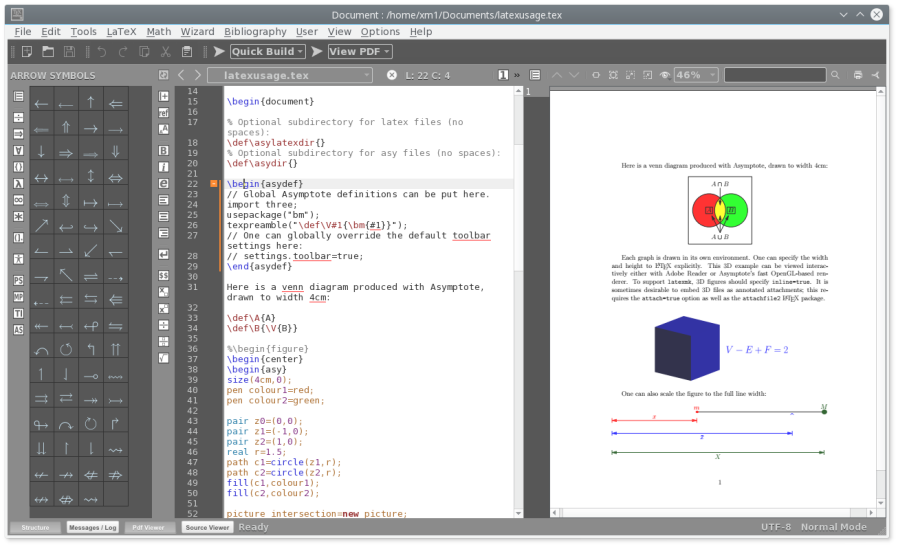
\includegraphics[width=\textwidth]{img/texmaker.png}
\end{frame}

\begin{frame}
  \frametitle{TeXMaker}
  \framesubtitle{Redigeringsprogram til \LaTeX}

  \begin{block}{\chref{https://www.xm1math.net/texmaker}{https://www.xm1math.net/texmaker}}
    \begin{itemize}
    \item Begyndervenlig editor til at skrive {\LaTeX} i
    \item Tilgængelig på GNU/Linux, macOS og Windows
    \item Fri software
    \end{itemize}
  \end{block}

  \begin{block}{Alternativer}
    \begin{itemize}
    \item TeXStudio (\chref{https://www.texstudio.org}{https://www.texstudio.org})
    \item Atom (\chref{https://atom.io}{https://atom.io})
    \item Emacs (\chref{https://www.gnu.org/software/emacs}{https://www.gnu.org/software/emacs})
    \item Hvilken som helst plain text editor
    \end{itemize}
  \end{block}
\end{frame}

\end{document}

%%% Local Variables:
%%% mode: latex
%%% TeX-master: t
%%% End:
